\chapter{Atmospheric Pressure}

The air you breathe is a blend of gases:
\begin{enumerate}
\item 78\% nitrogen in the form of $N_2$
\item 21\% oxygen in the form $O_2$
\item 1\% other gases (mostly argon)
\end{enumerate}

If you fill a balloon with helium ($He$),  the helium will push against the interior of the balloon with some pressure.   
The pressure is the same at every point in the interior of the balloon.  Pressure,  then,  is force spread over some area.   
Force is commonly measured in newtons.   Pressure is measured in \newterm{pascals}.  A pascal is 1 newton per square meter.\index{pressure}

We don't usually think about it,  but the air outside the balloon is also pushing against the exterior of the balloon.  
We call this \newterm{barometric pressure} or \newterm{atmospheric pressure} and it is caused by gravity pulling on the gas molecules above the balloon.\index{barometric pressure}\index{atmospheric pressure}

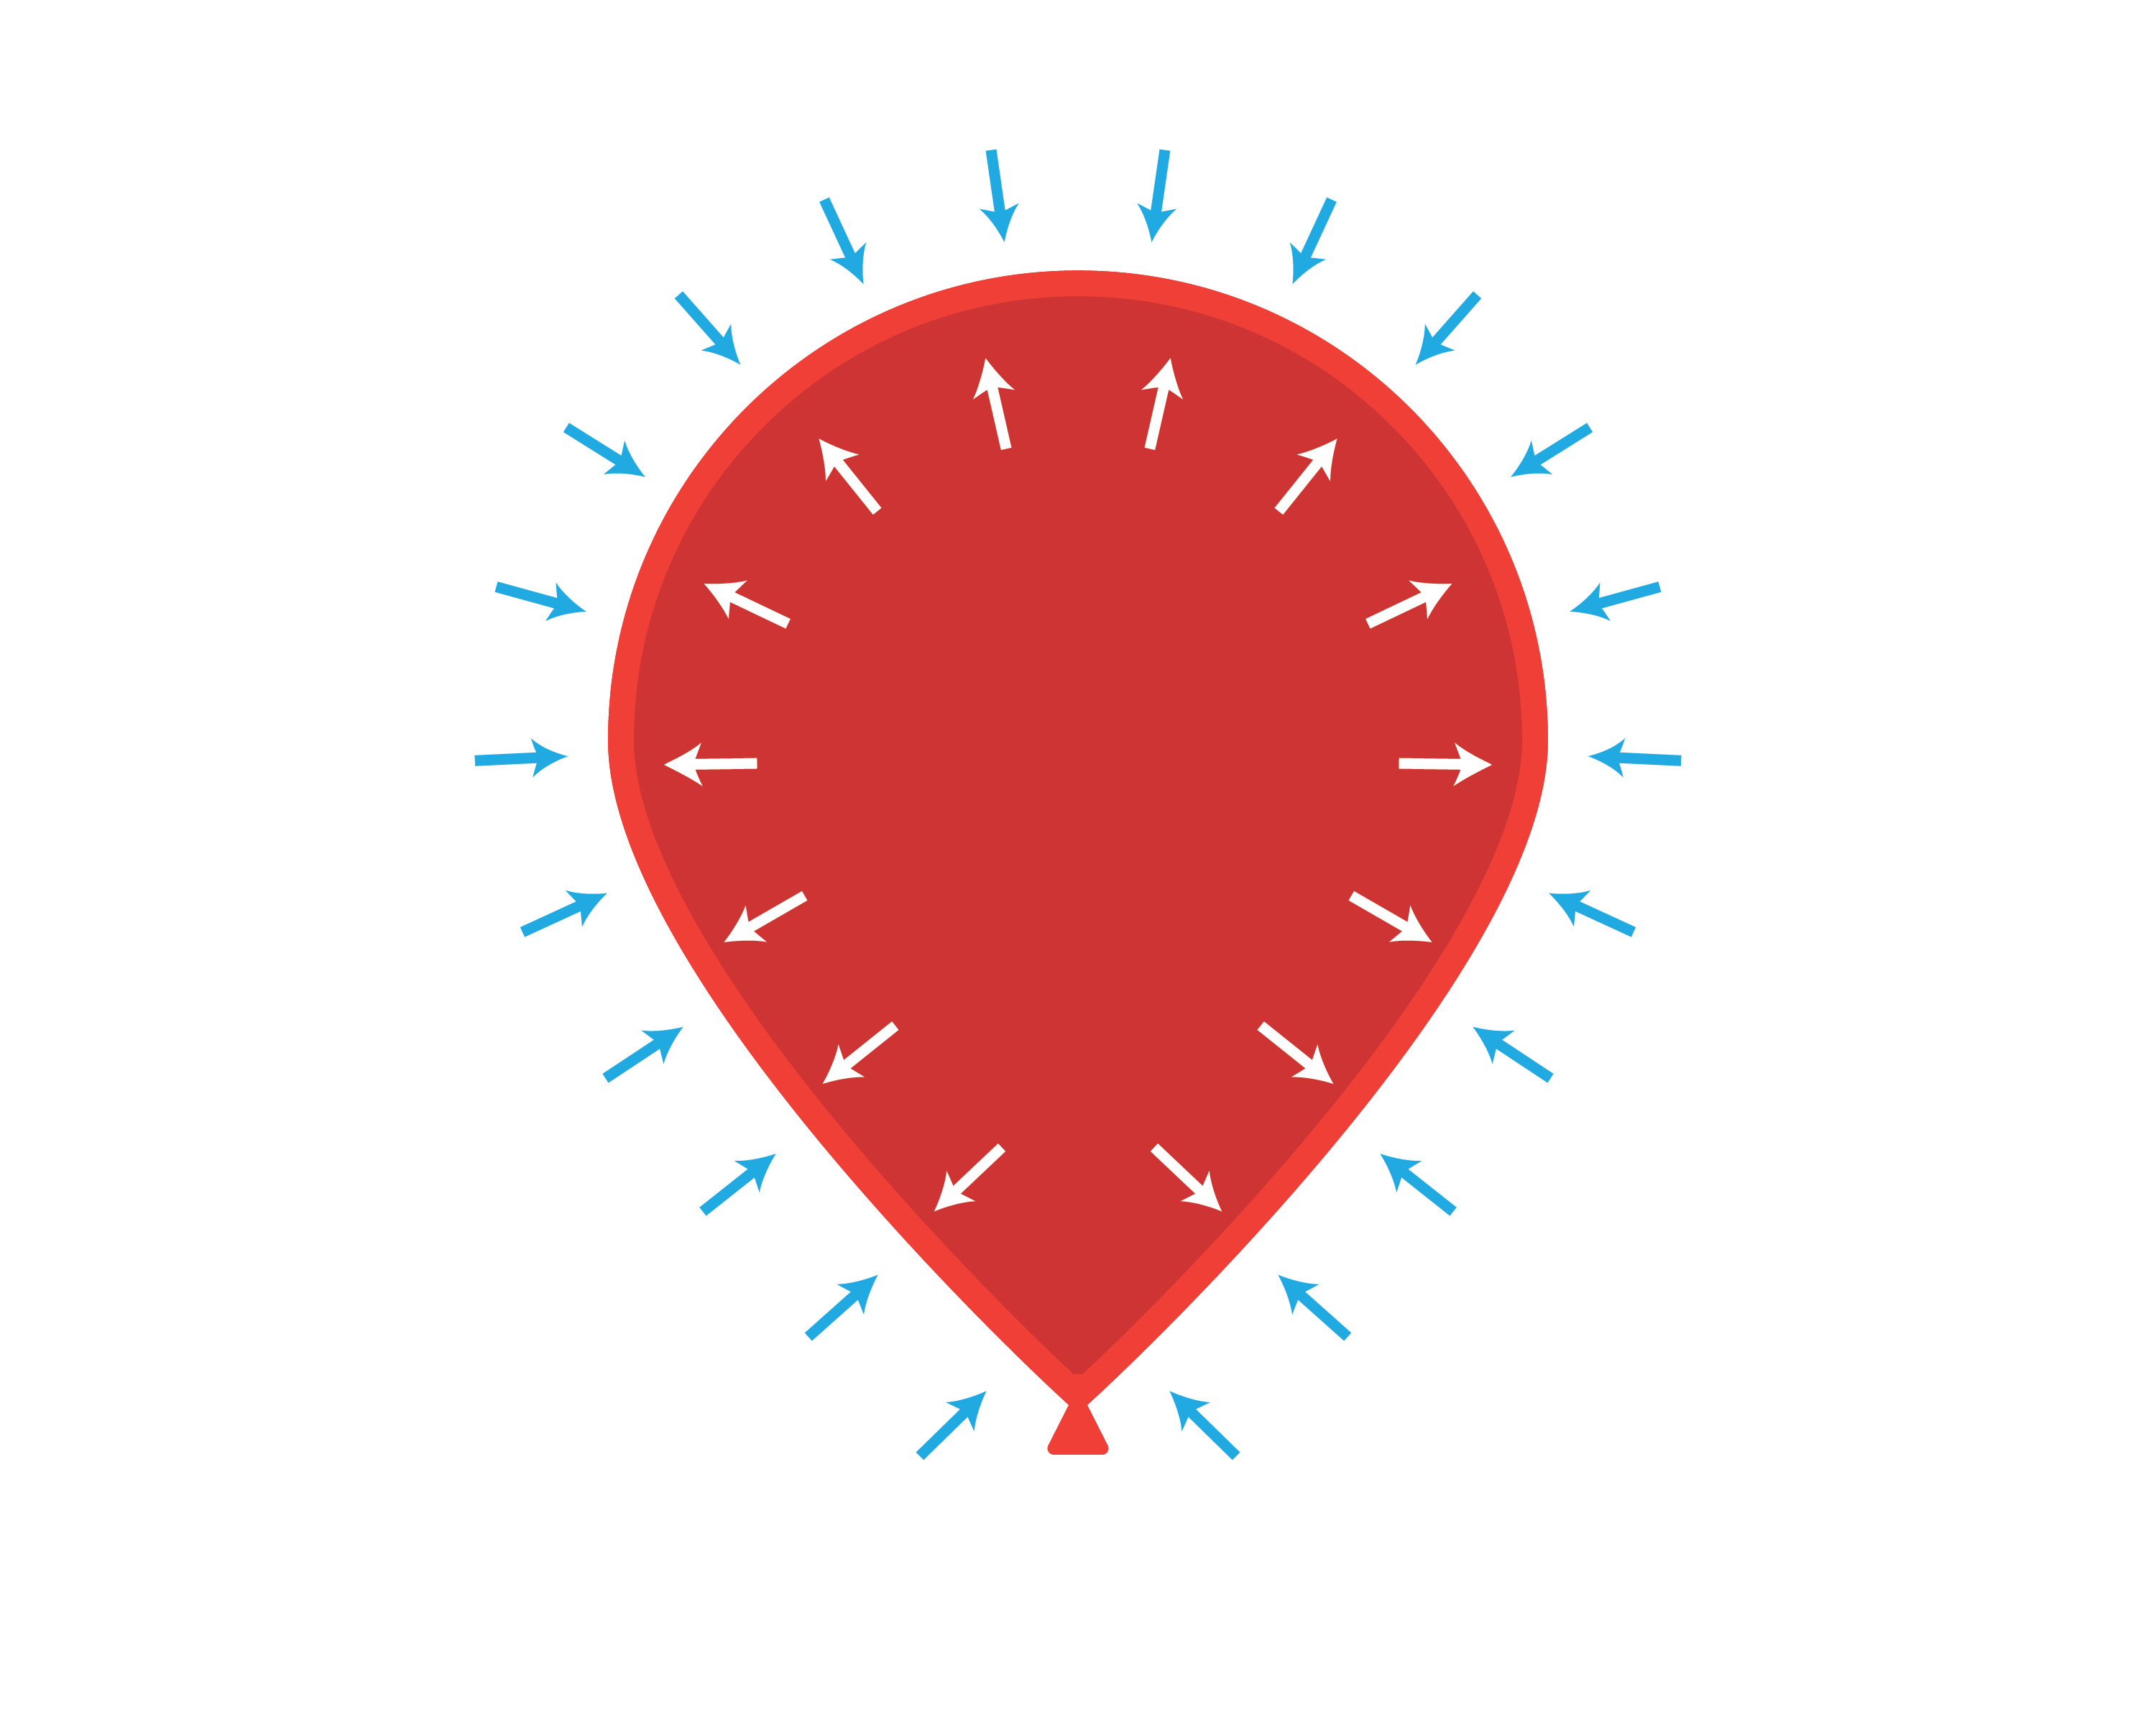
\includegraphics[width=\textwidth]{balloon.png}


Imagine a square meter on the ground at sea level.  Now imagine the column of air above it -- reaching all the way to the top of the atmosphere.

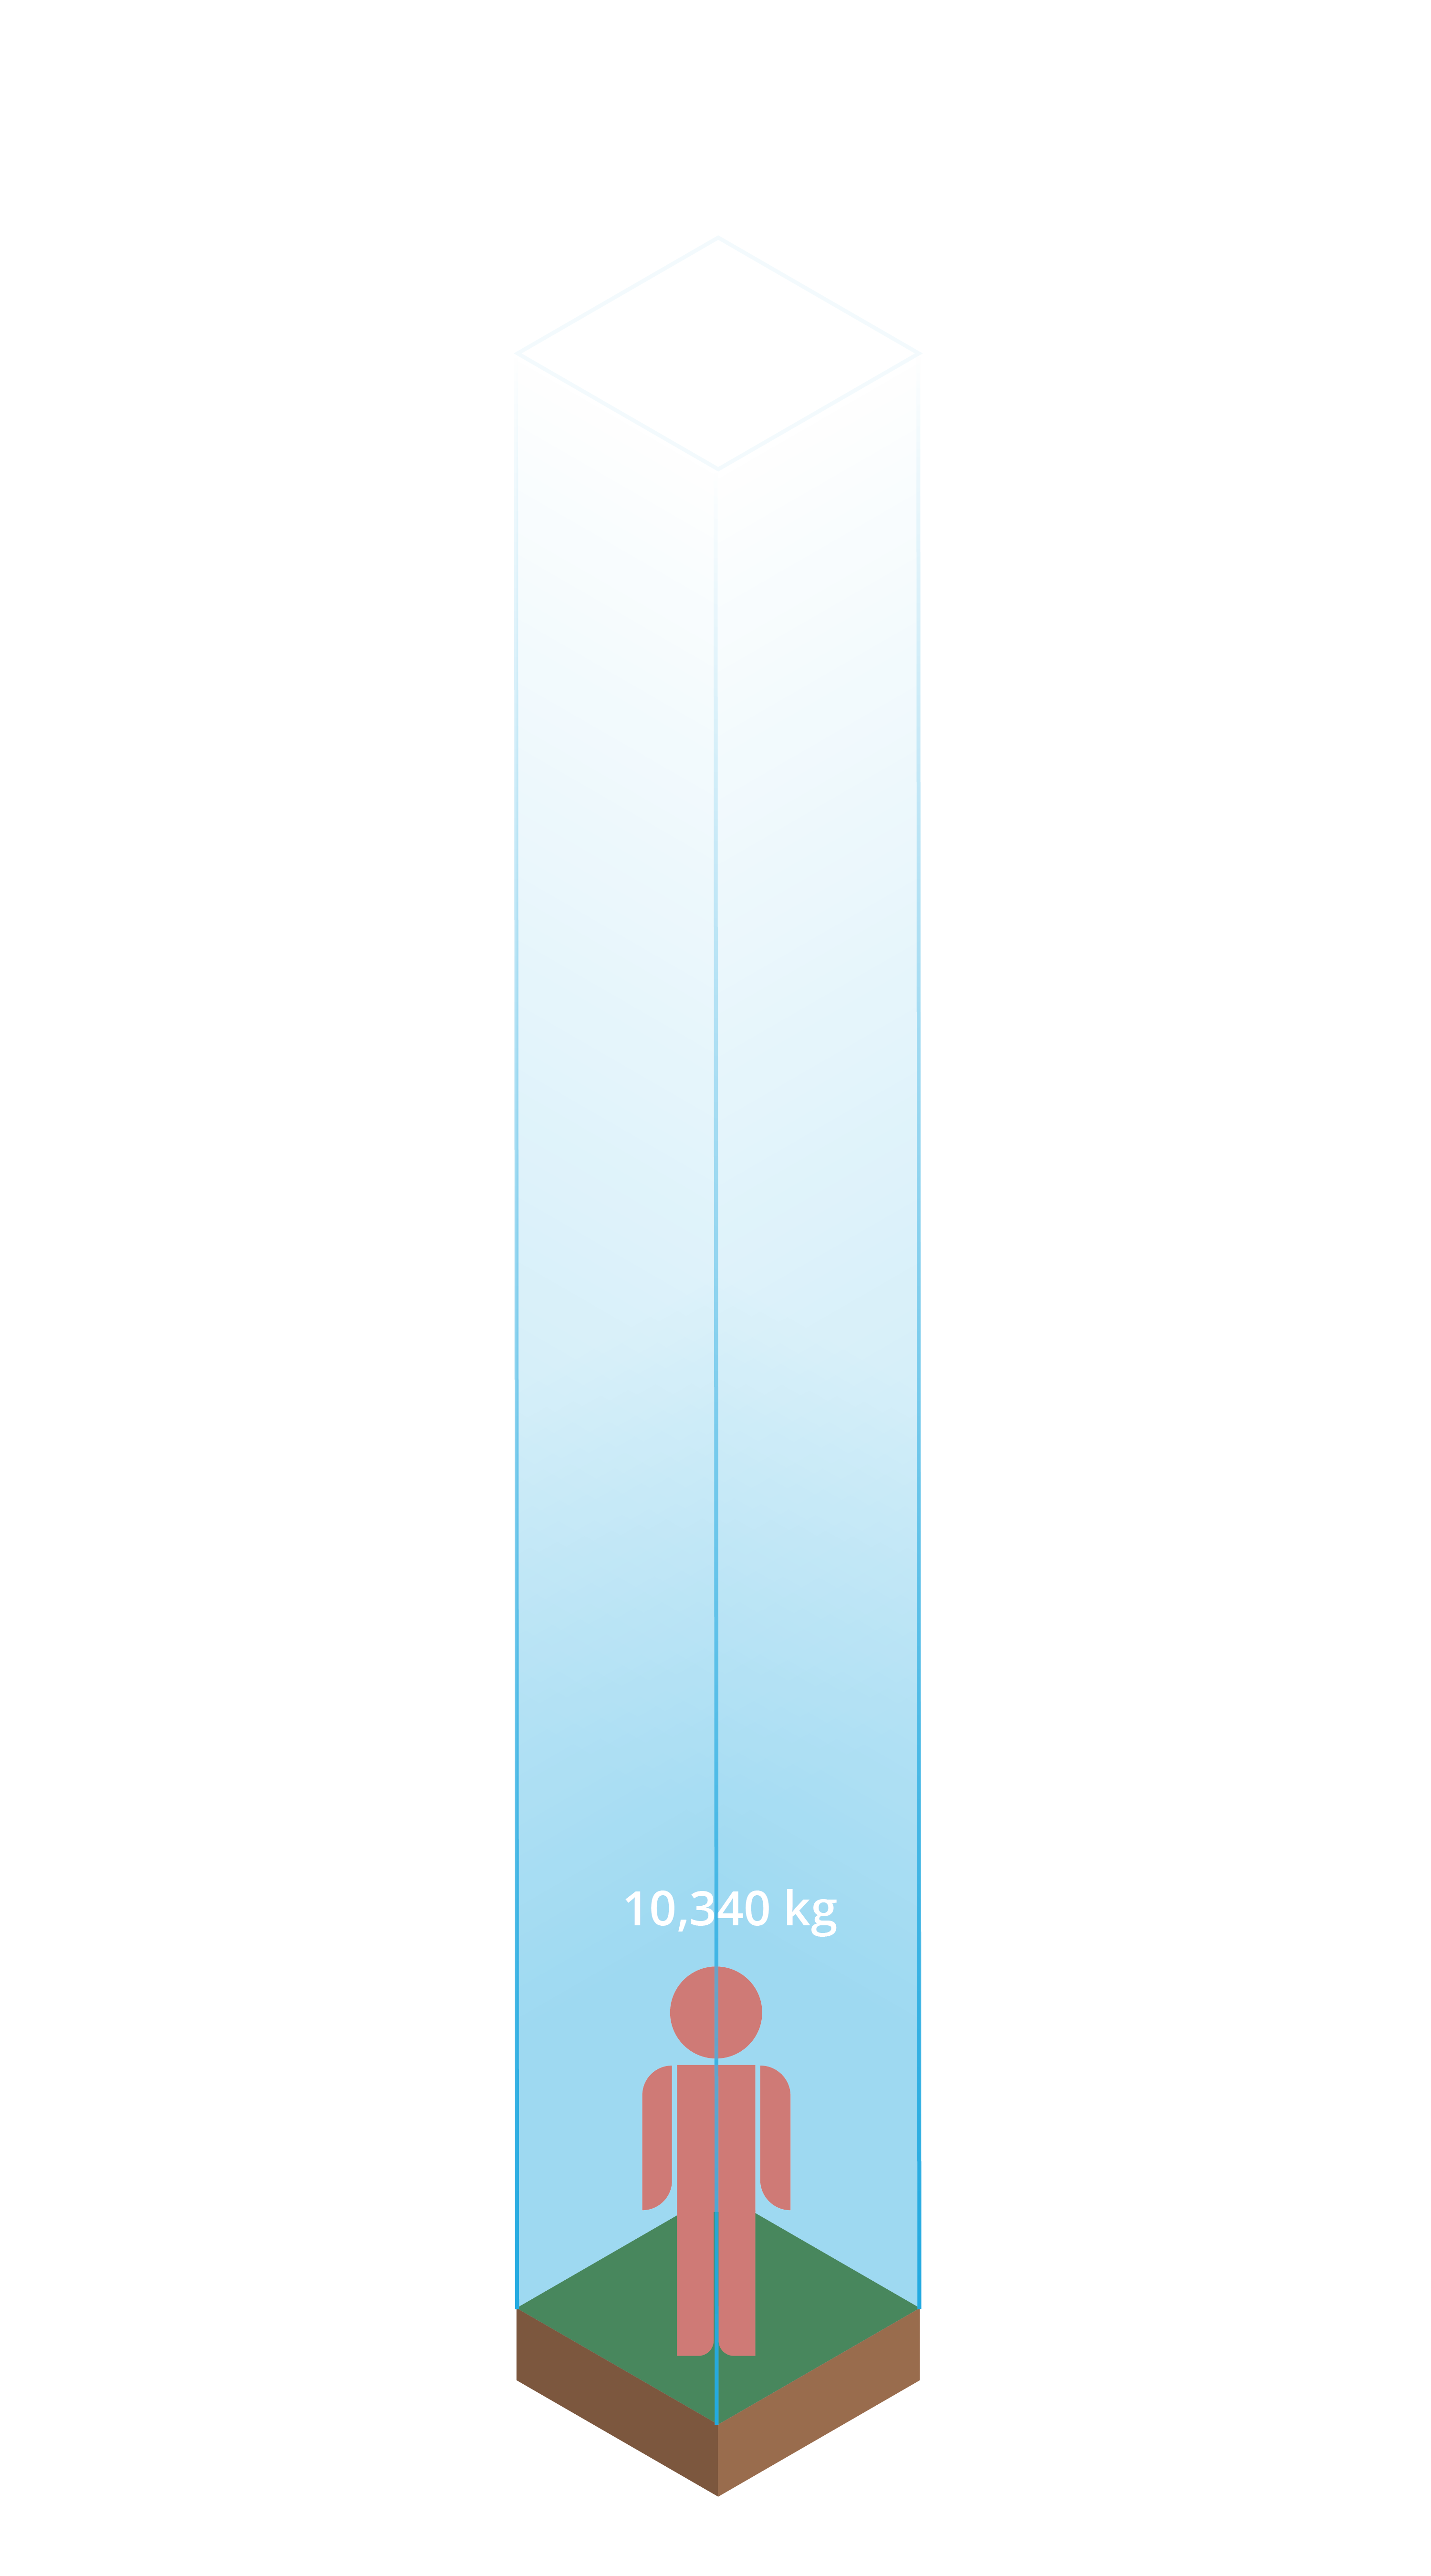
\includegraphics[width=\textwidth]{aircolumn.png}

The air inside that column has a mass of about 10,340 kg.  One kilogram on the earth experiences a gravitational force of 9.8 N.   
So the atmospheric pressure all around you is about 101,332 pascals.  
When dealing with such large numbers, we often use kilopascals.  
We'd say the barometric pressure at sea level is about 101.3 kPa.

That's a lot of pressure!  Why doesn't your ribcage collapse crushing your lungs?  The air \emph{inside} your lungs is the same 
pressure as the air push on the outside of your rib cage.  

And thus we live pretty much oblivious to this huge force that is all around us, but you can see it sometimes.  
For example, if you suck the air out of a plastic bottle,   the bottle will be crushed by the barometric pressure.

\section{Altitude and Atmospheric Pressure}

If you let go of the balloon, as it rises through this column there will be less and less air mass above it, and thus less and less atmospheric pressure on the outside of the balloon. While the pressure pushing against the outside of the balloon decreases, the interior pressure causes the balloon to expand. The balloon will continue to grow as it rises until it stretches so far that it rips and pops.


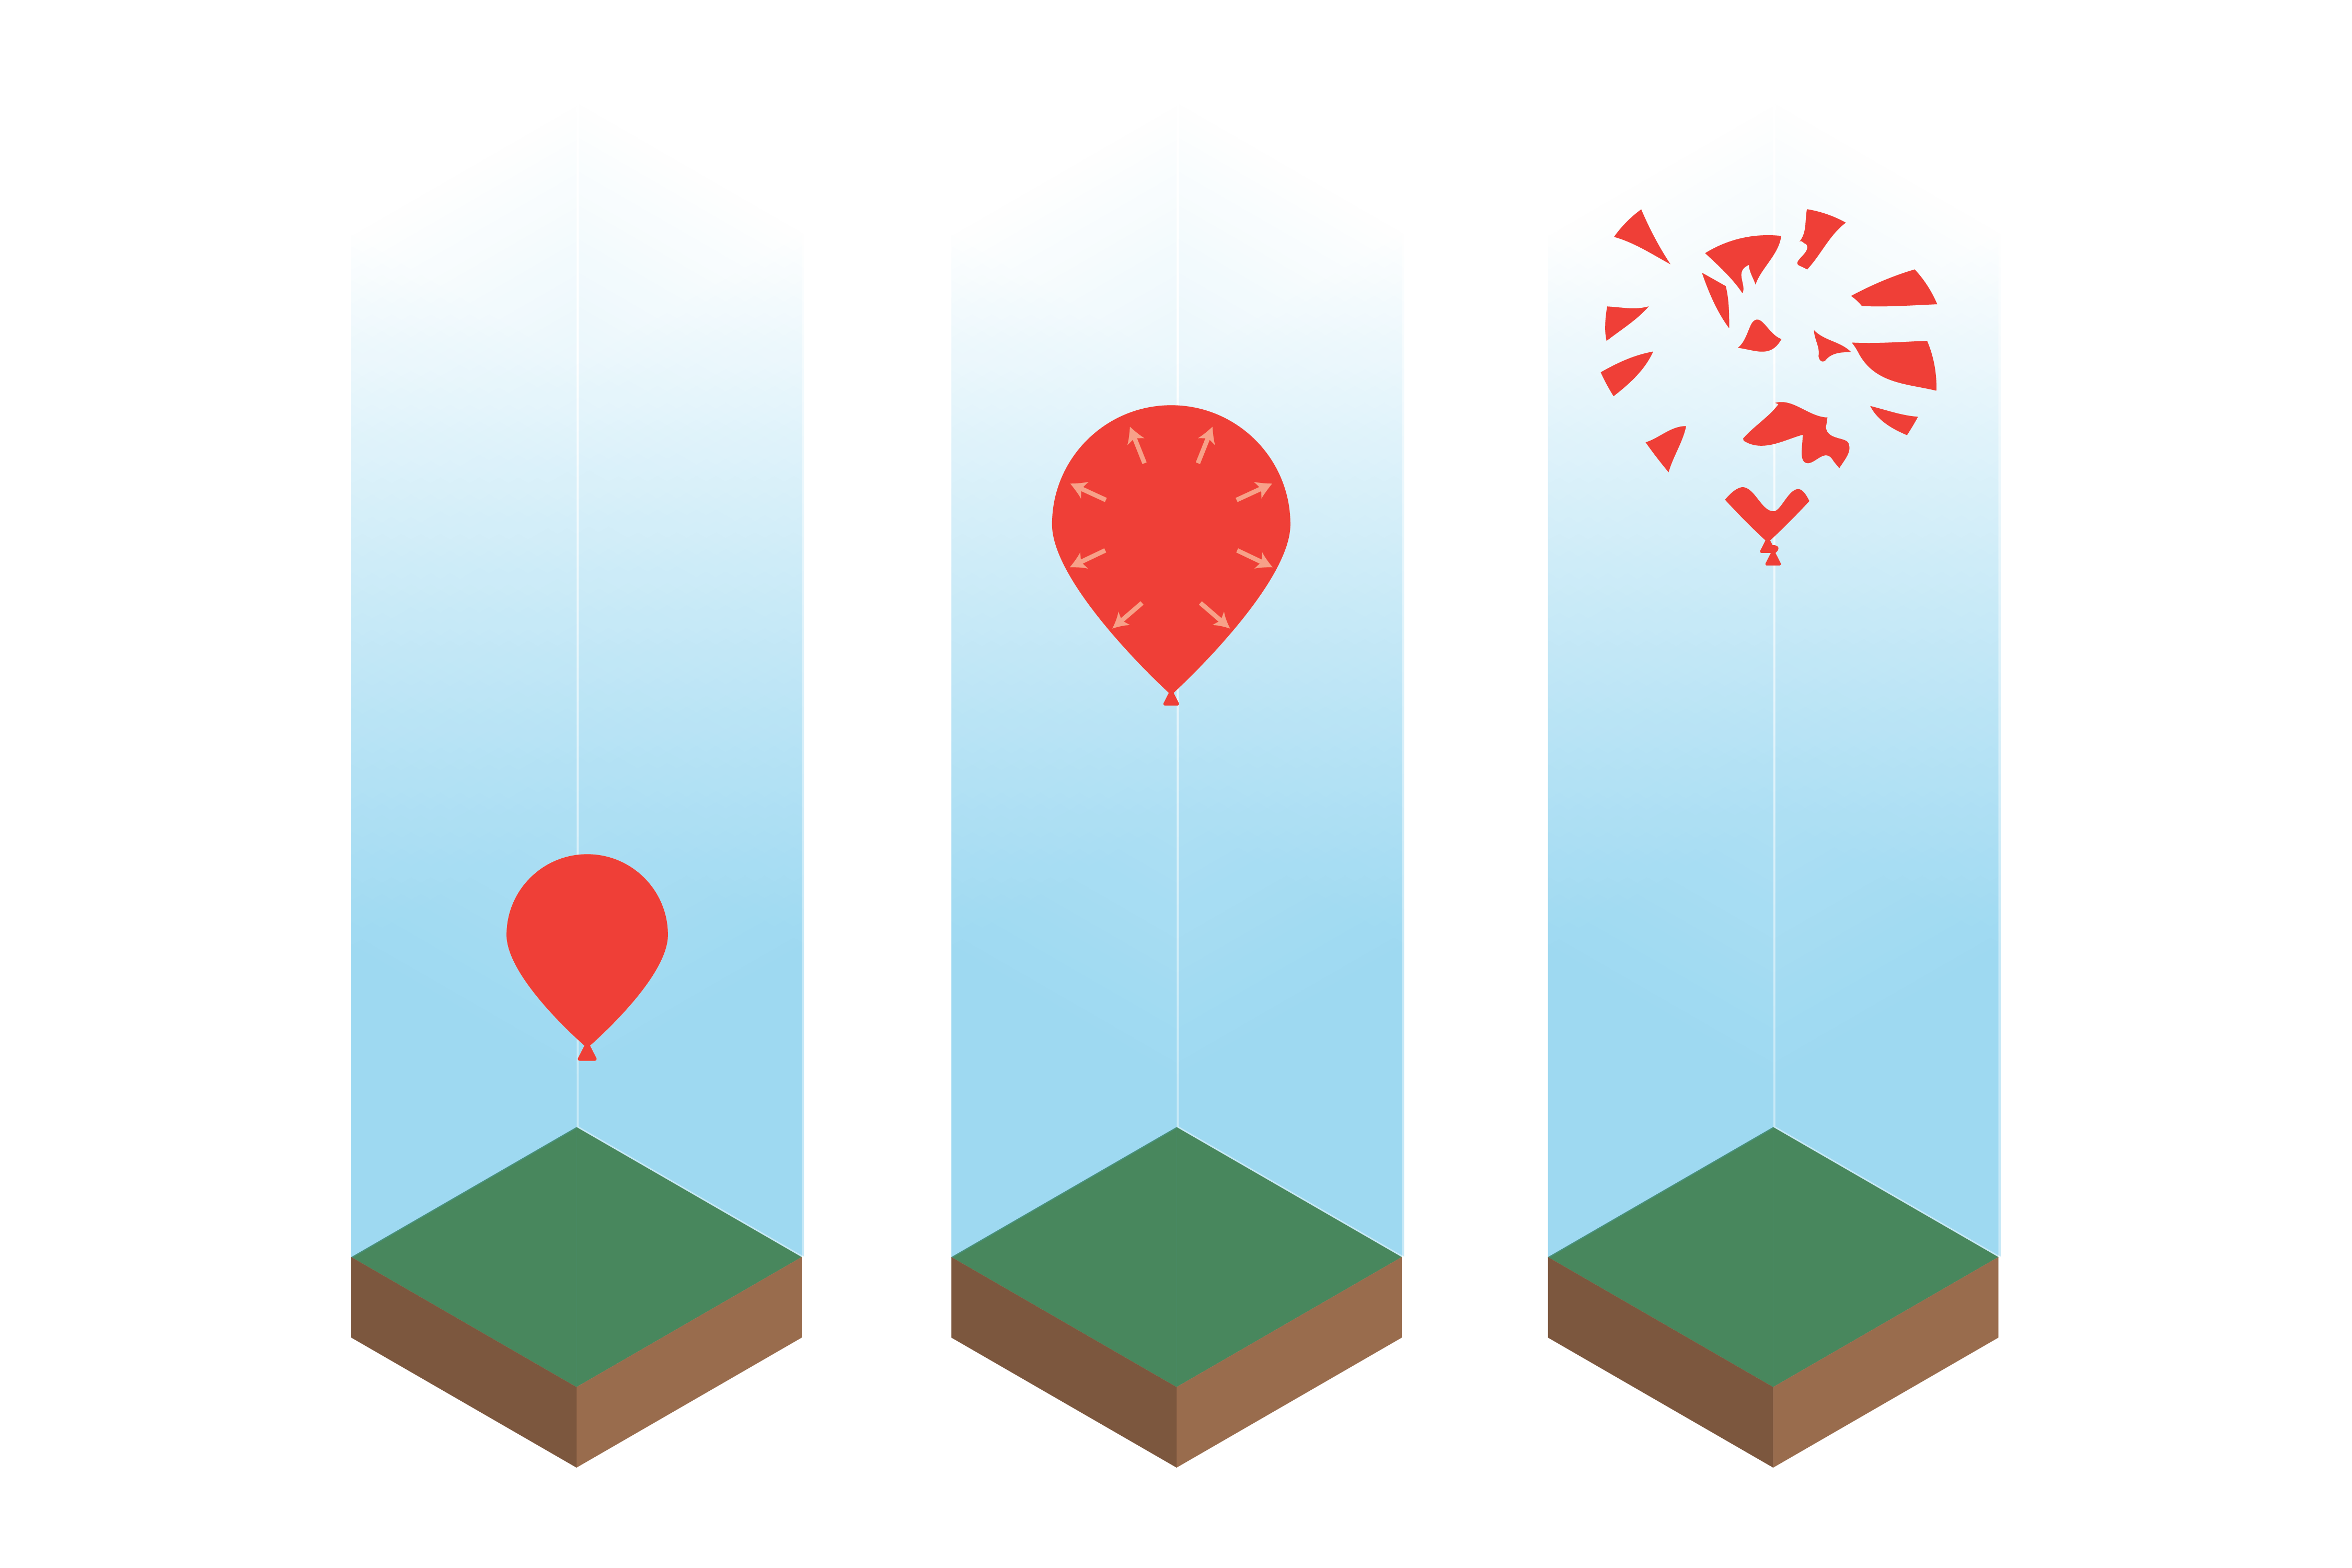
\includegraphics[width=\textwidth]{balloonColumn.png}

What would be the atmospheric pressure at $h$ meters above sea level?  Here is a handy formula for that:

$$p = 101,332 \times \left(1 - \left( 2.25577 \times 10^{-5} \times h\right) \right)^{5.25588}$$

where $p$ is the atmospheric pressure in pascals.

\begin{Exercise}[title={Atmospheric Pressure},  label=atmos_pressure]
  
You are thinking about riding your bicycle to the top of Mount Everest.  You are worried when the atmospheric pressure outside the tire drops,  the tire will fail.  
(I have had a tire fail before; It is very, very loud.)  

Calculate the atmospheric pressure at the top of Mount Everest (9,144 meters above sea level).

\end{Exercise}
\begin{Answer}[ref=atmos_pressure]

$$p = 101,332 \times \left(1 - 2.25577 \times 10^{-5} \times h\right)^{5.25588}$$

and $h = 9,144$.  Thus,

$$p \approx 30.1 \text{kPa}$$

\end{Answer}

\section{How a Drinking Straw Works}

When you suck on a drinking straw,  why does the beverage rise?  
It is actually pushed by atmospheric pressure.

Before you put your mouth on the straw,  the atmospheric pressure is pressing on the 
entire surface of the liquid (even inside the straw) evenly.   Gravity pulls on the liquid making the surface
level.

When you suck some air out of the straw,  the pressure on the surface inside the straw drops.  The atmospheric pressure on the surface outside the straw pushes into the straw and the beverage rises.

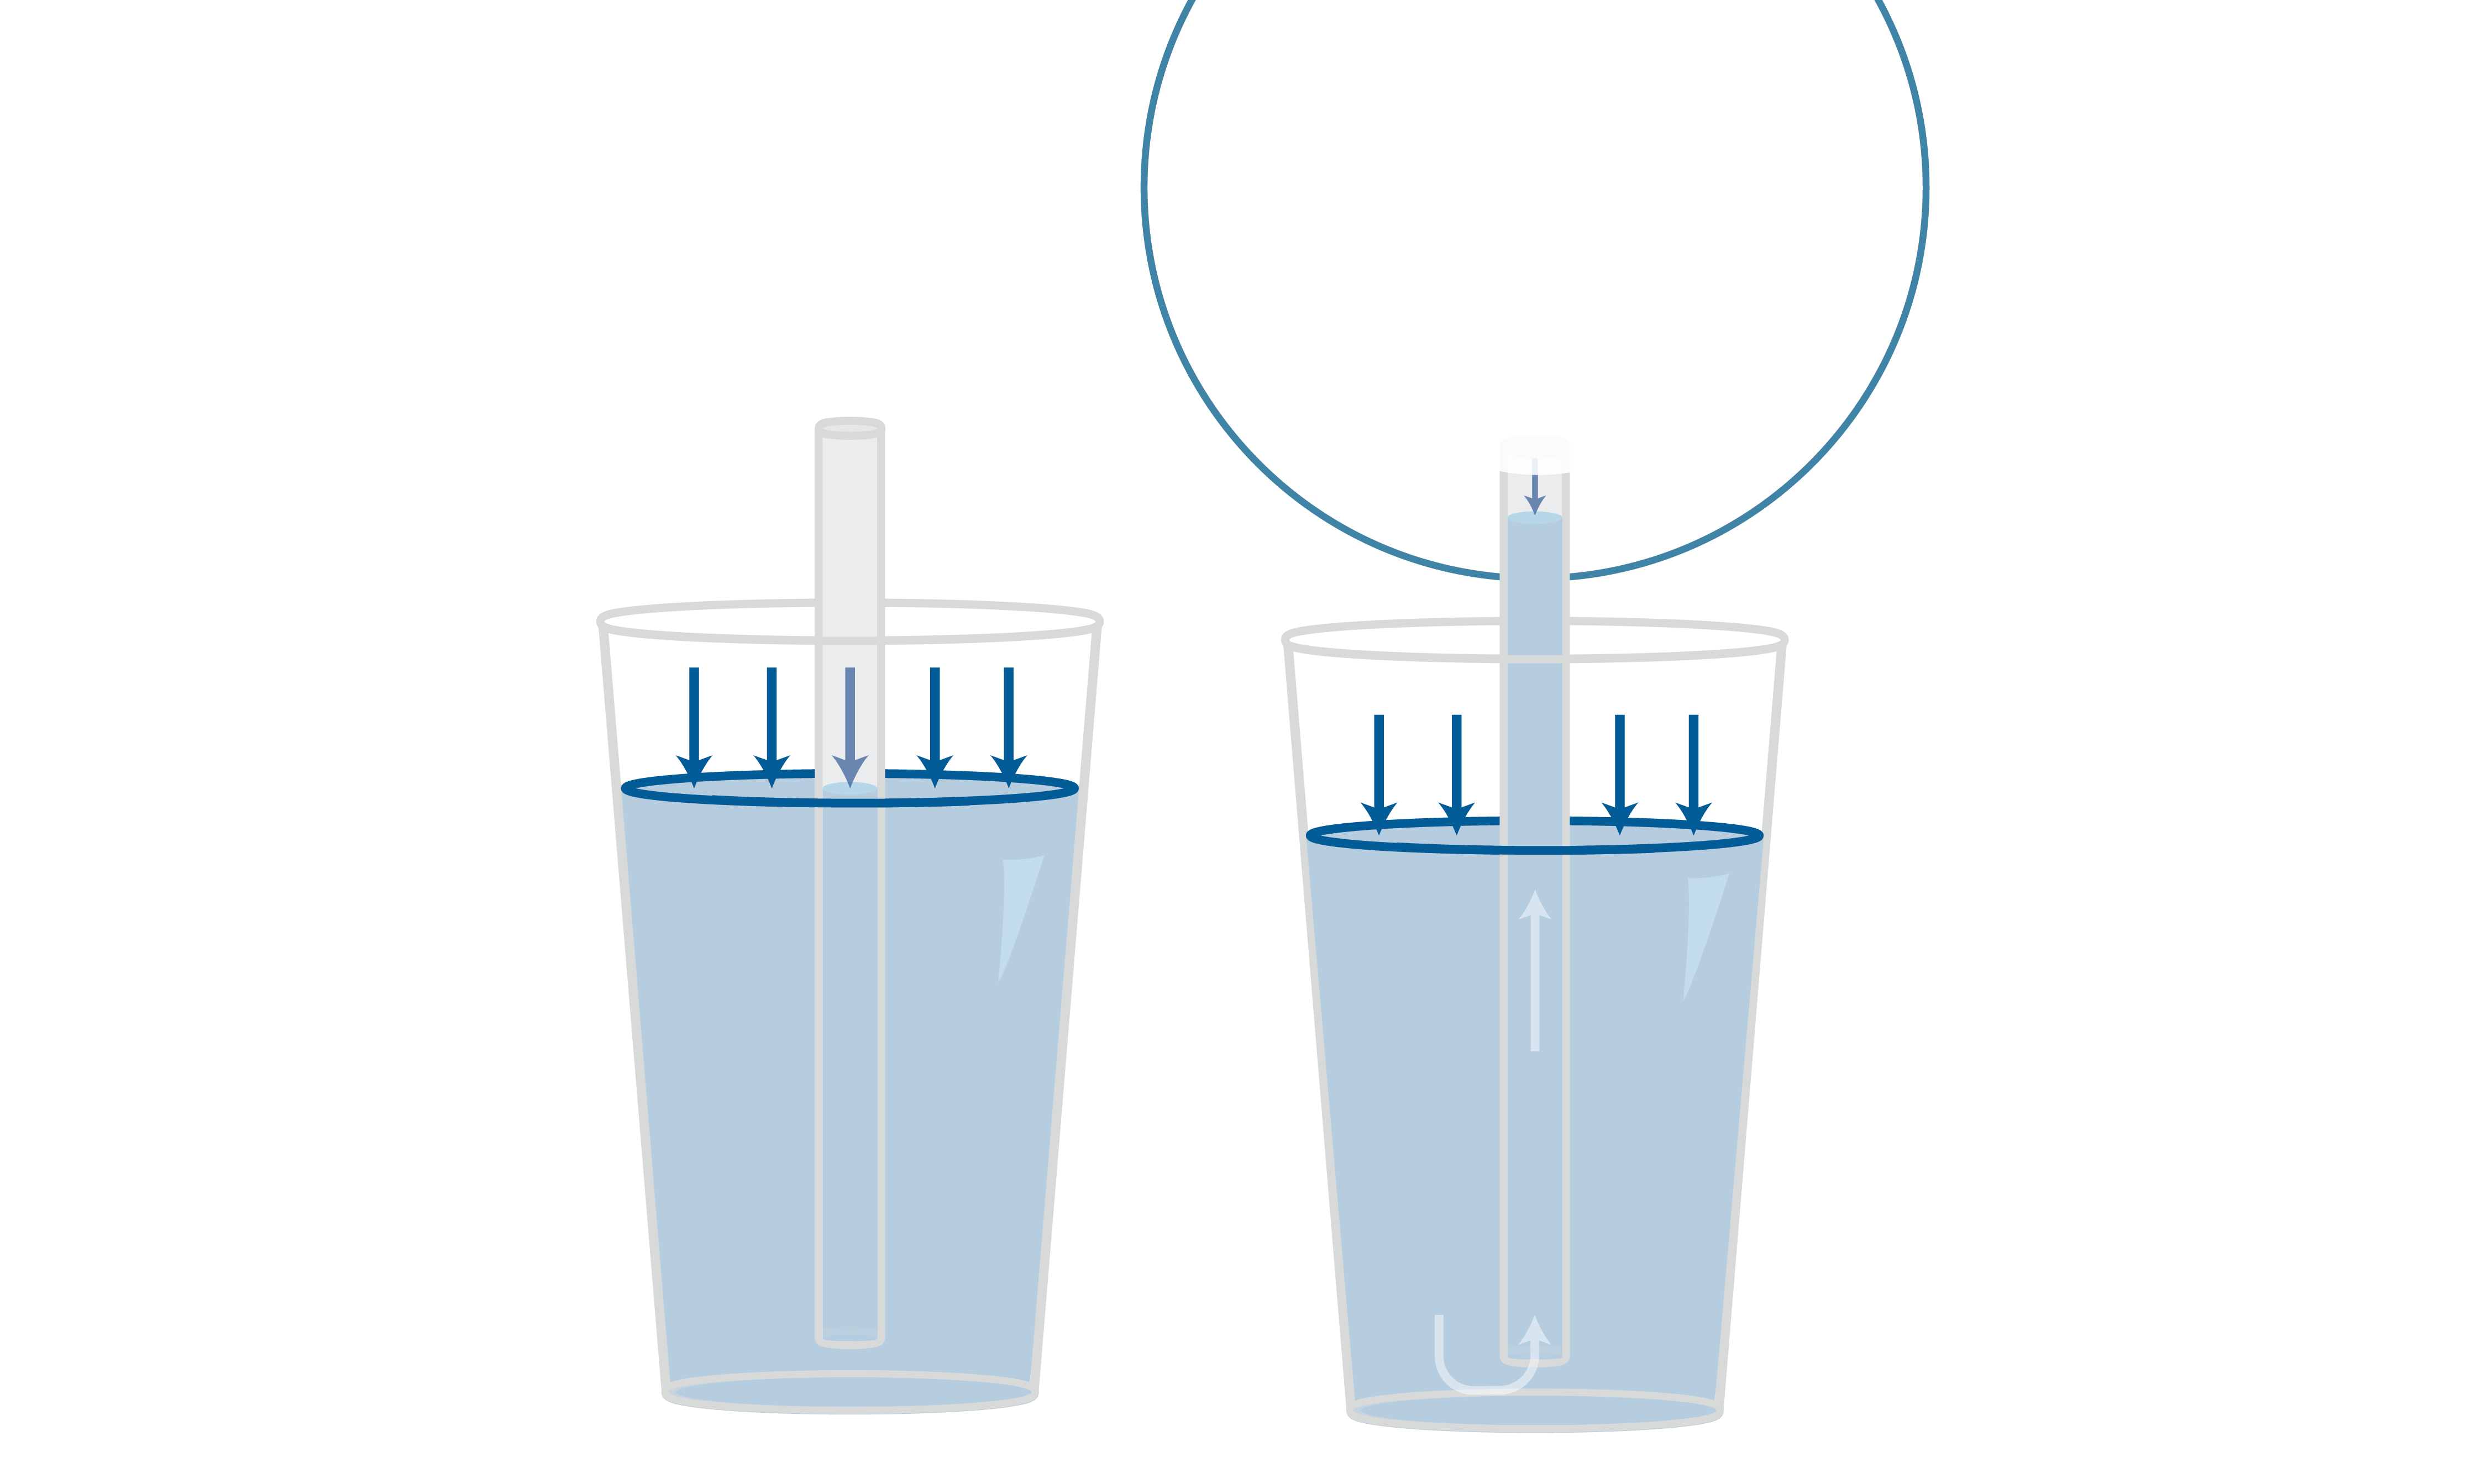
\includegraphics[width=\textwidth]{straw.png}


Of course,  gravity is still trying to pull the liquid inside the straw back down.  And for every inch that you lift the liquid in the straw,  the force of gravity gets greater, demanding more suction.

\subsection{The Longest Usable Straw}
  
Assuming you are drinking water in a place with 100 kPa of atmospheric pressure,   how high could 
you suck water with a perfect vacuum?  That is,  given a very, very long and very, very stiff drinking straw,  if you created a pressure of 0 Pa inside,  how far above the surface of the glass 
could you get the water? \index{straw!drinking}

Let's say a cross-section of the straw has an area of $a$ square meters and the very top of the 
column of water is $h$ meters above the surface in the glass. 

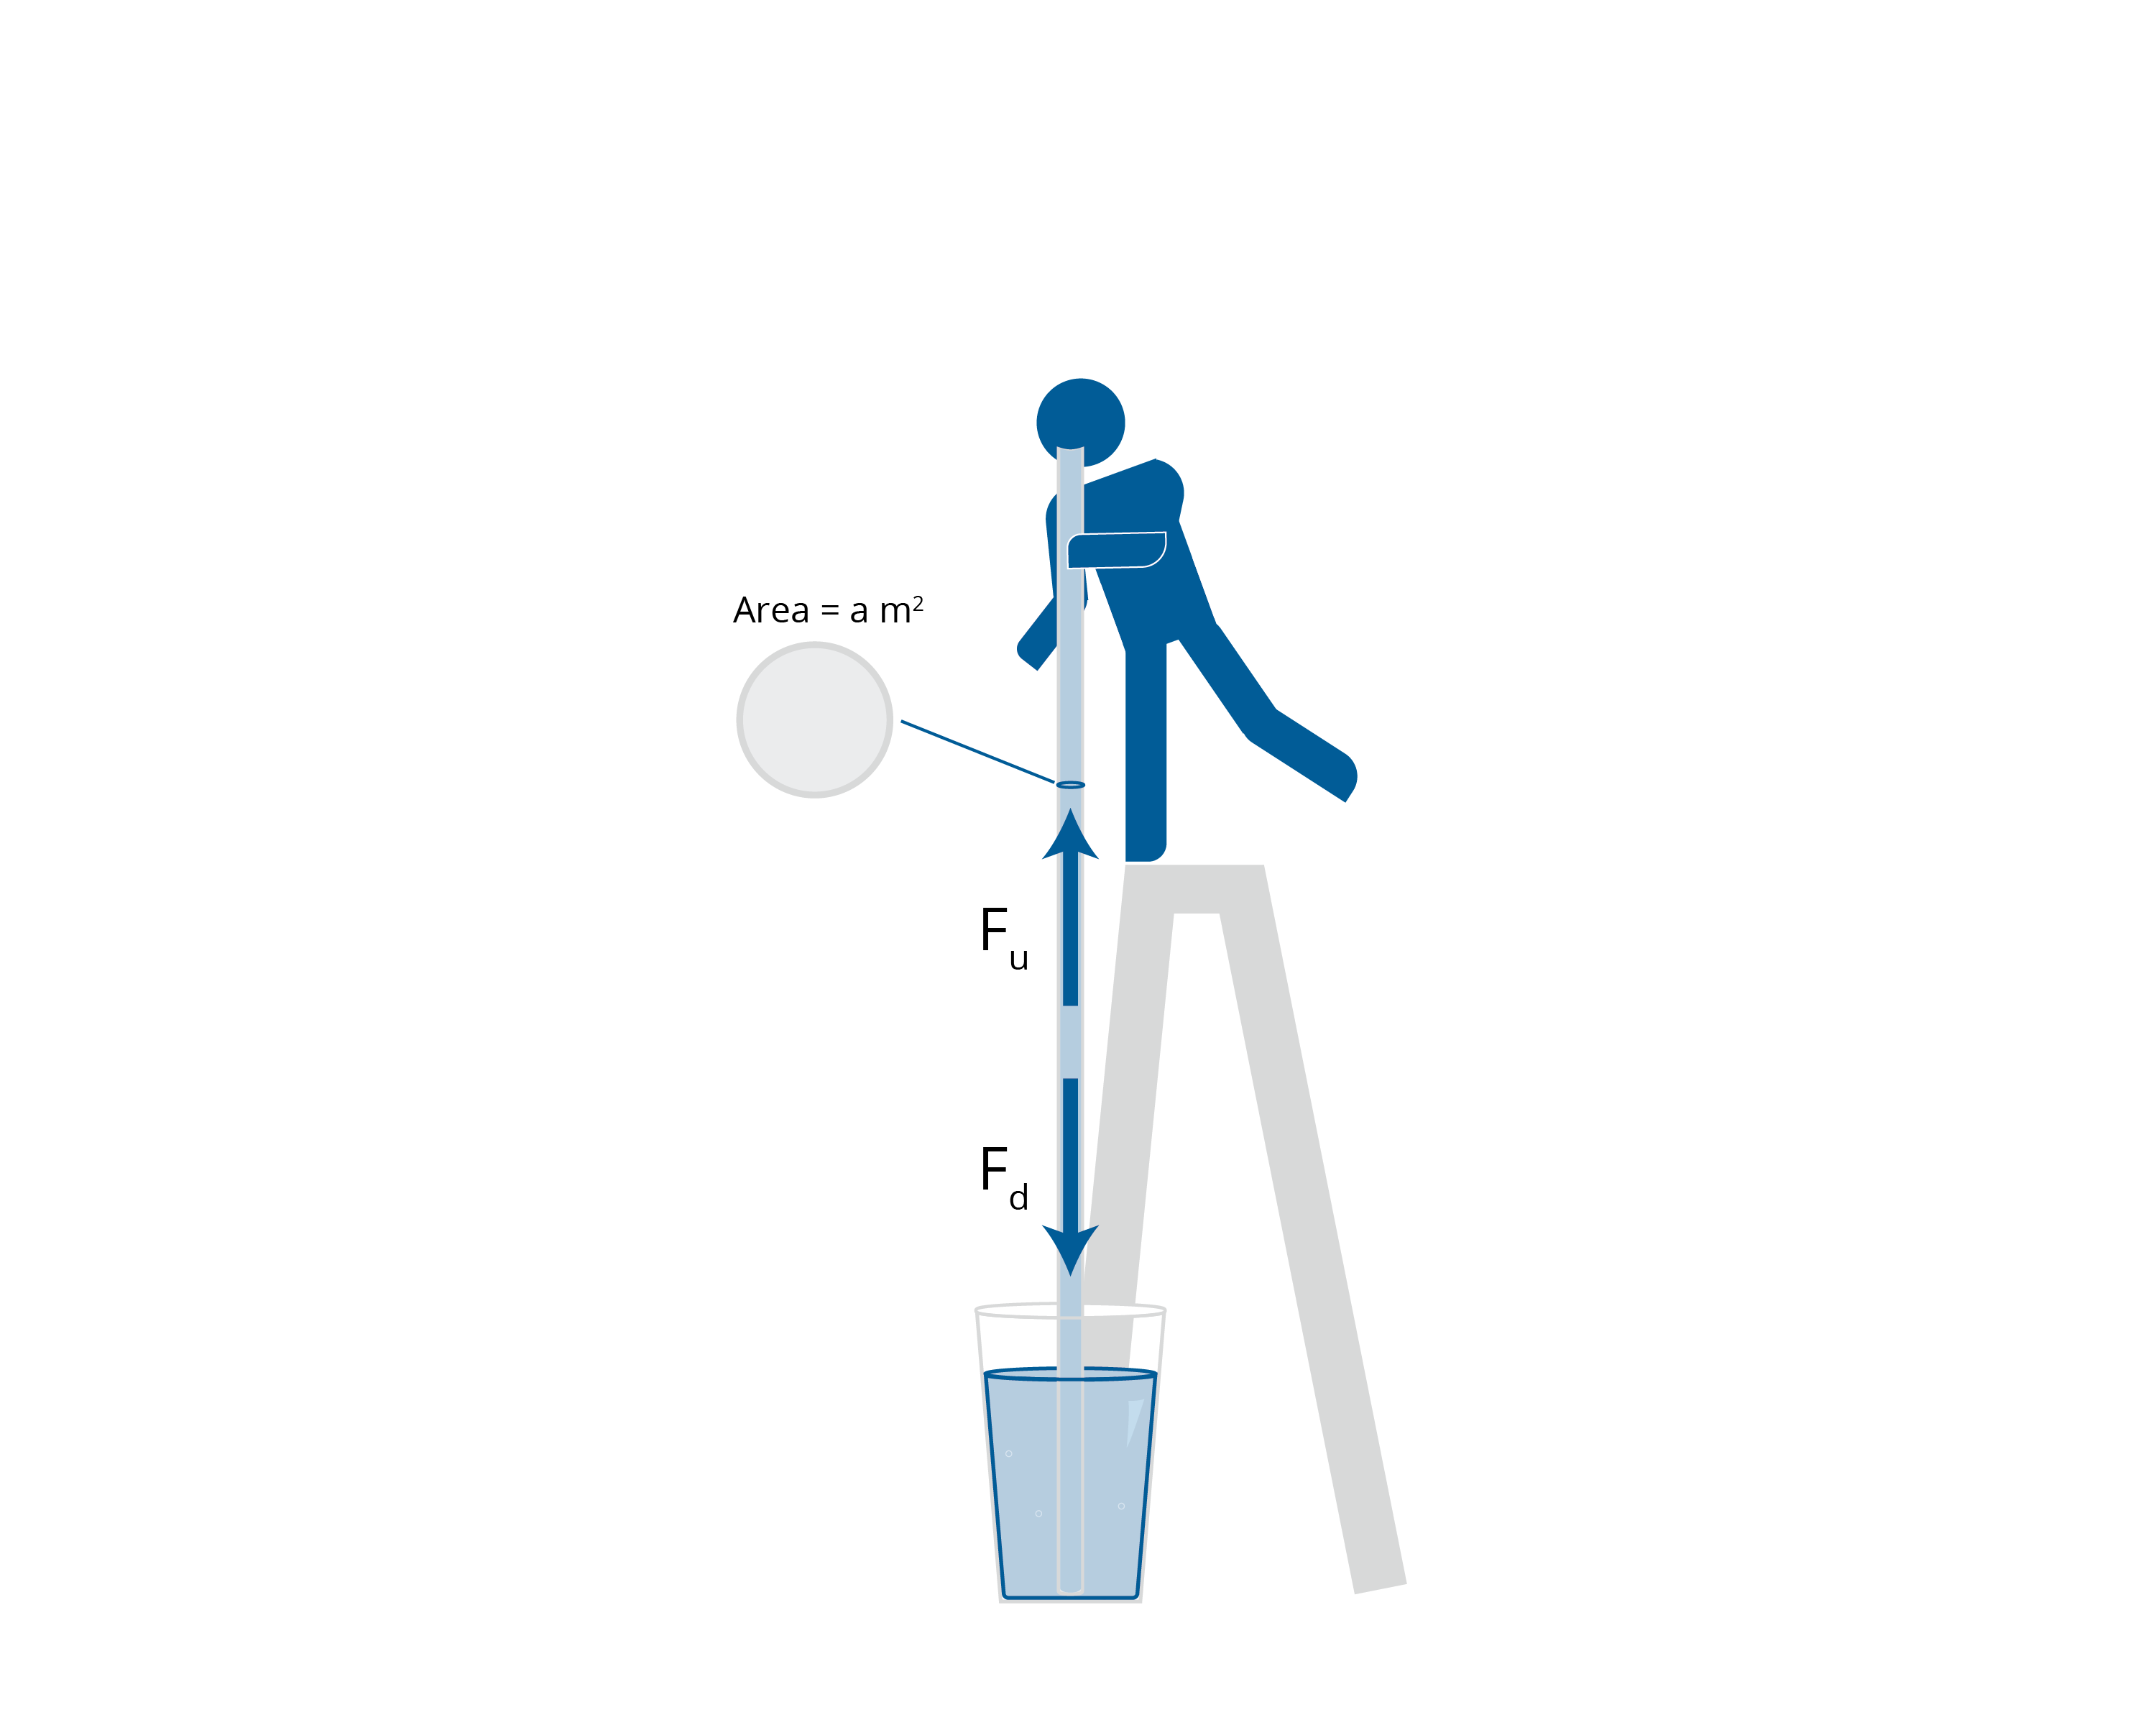
\includegraphics[width=\textwidth]{tallStraw.png}


With how many newtons of force is the atmosphere pushing the water upward?  100 kPa = 100,000 newtons per square meter.  So:

$$F_u = (100,000)a$$

With many newtons of force is gravity pulling the water in the straw downward?  The volume of the water is $ah$.  A cubic meter of liquid water weights 1000 kg.  The force of gravity is 9.8 Newtons per kg.

$$F_d = (ah)(1000)(9.8)$$

The water will stop rising when $F_u = F_d$.  So to find $h$ we substitute in:

$(100,000)a = (ah)(1000)(9.8)$

Notice that we can divide both sides by $a$ getting:

$$h = \frac{100,000}{9,800} = 10.2 \text{ meters}$$

A perfect vacuum would only be able to drag the water up 10.2 meters.

\subsection{Millimeters Mercury}

The density of mercury is 13,500 kg per cubic meter.  How far up a straw would a perfect vacuum pull mercury? \index{millimeters mercury}

$$h = \frac{100,000}{(9.8)(13,500)} \approx 0.756 \text{ meters}$$

That is, when the atmospheric pressure is 100kPa,  the mercury will rise 756 mm into a vacuum.

This is actually how scientists measure atmospheric pressure.   They have a long glass tube filled with mercury.  One end is closed off and pointed into the sky (exactly opposite the direction of gravity).  The other end is placed into a dish of mercury.  There are millimeter marks on the glass tube.

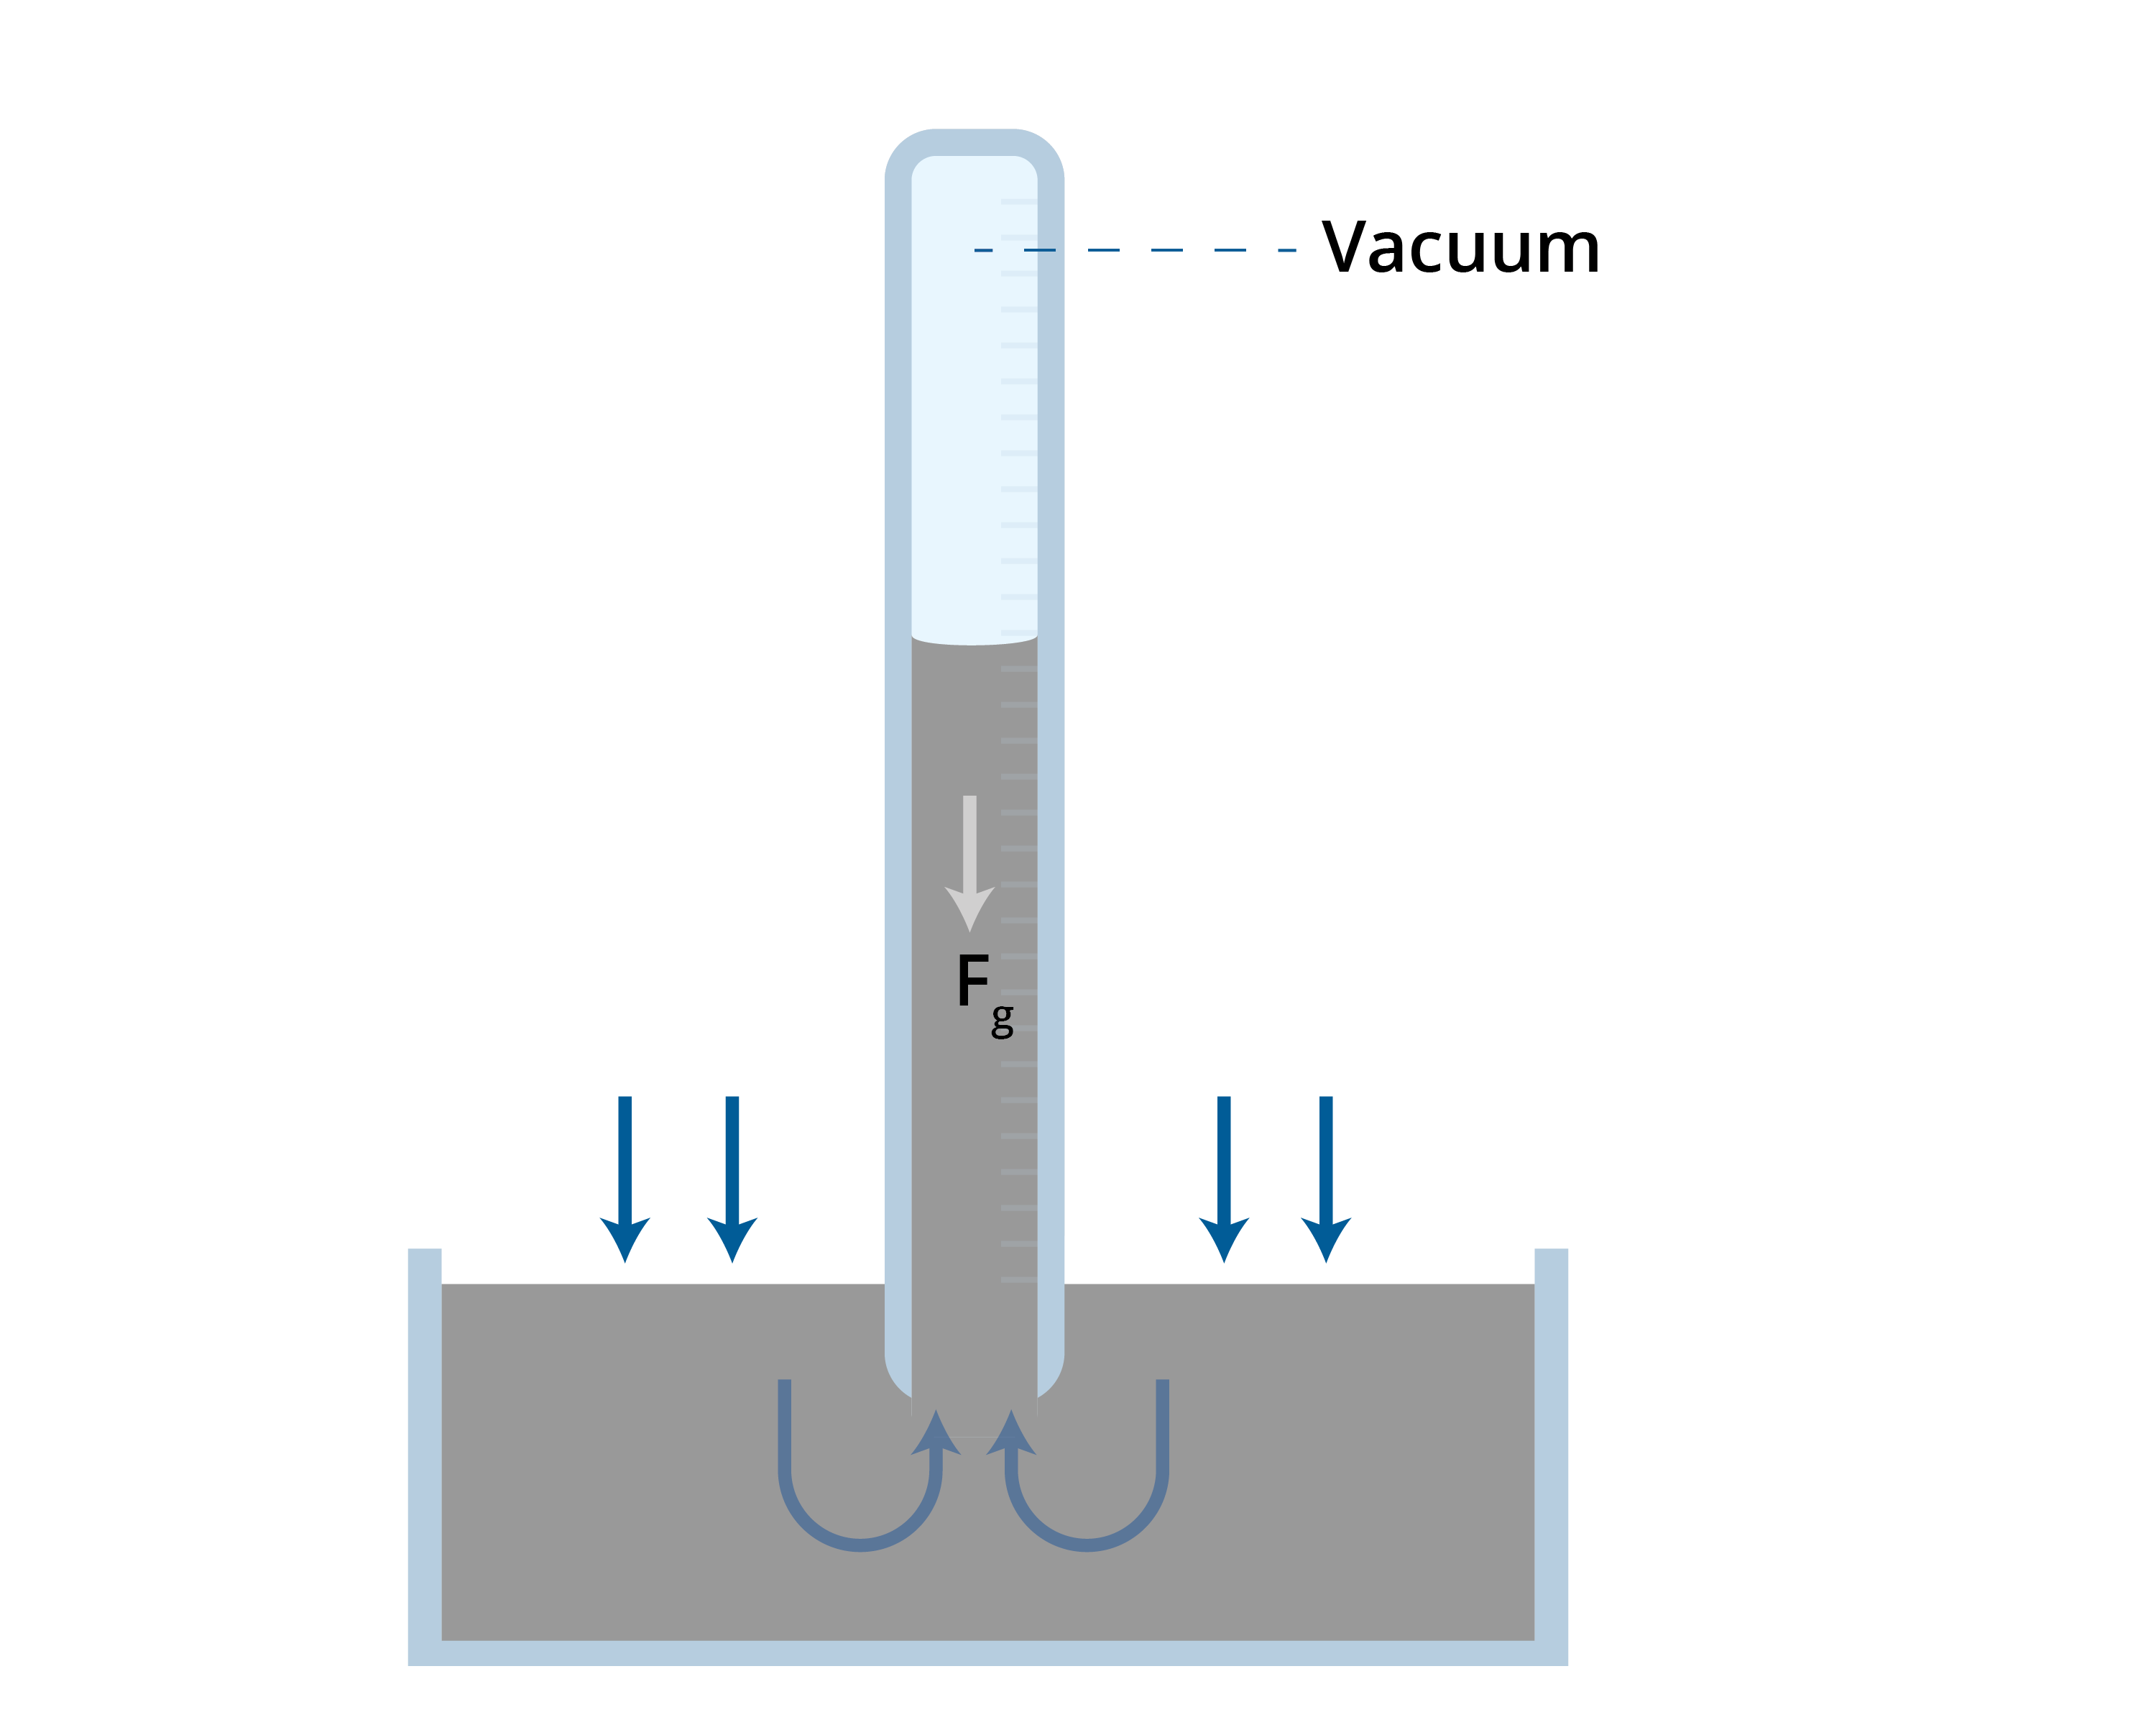
\includegraphics[width=\textwidth]{barometer.png}


We use fluctuations in the atmospheric pressure to help us predict the weather.  You might hear a weather nerd with a barometer in his house say, "Wow, the barometer has gone from 752 to 761 millimeters mercury in the last hour.  A high-pressure system is moving in." 


\section{How Siphon Works}

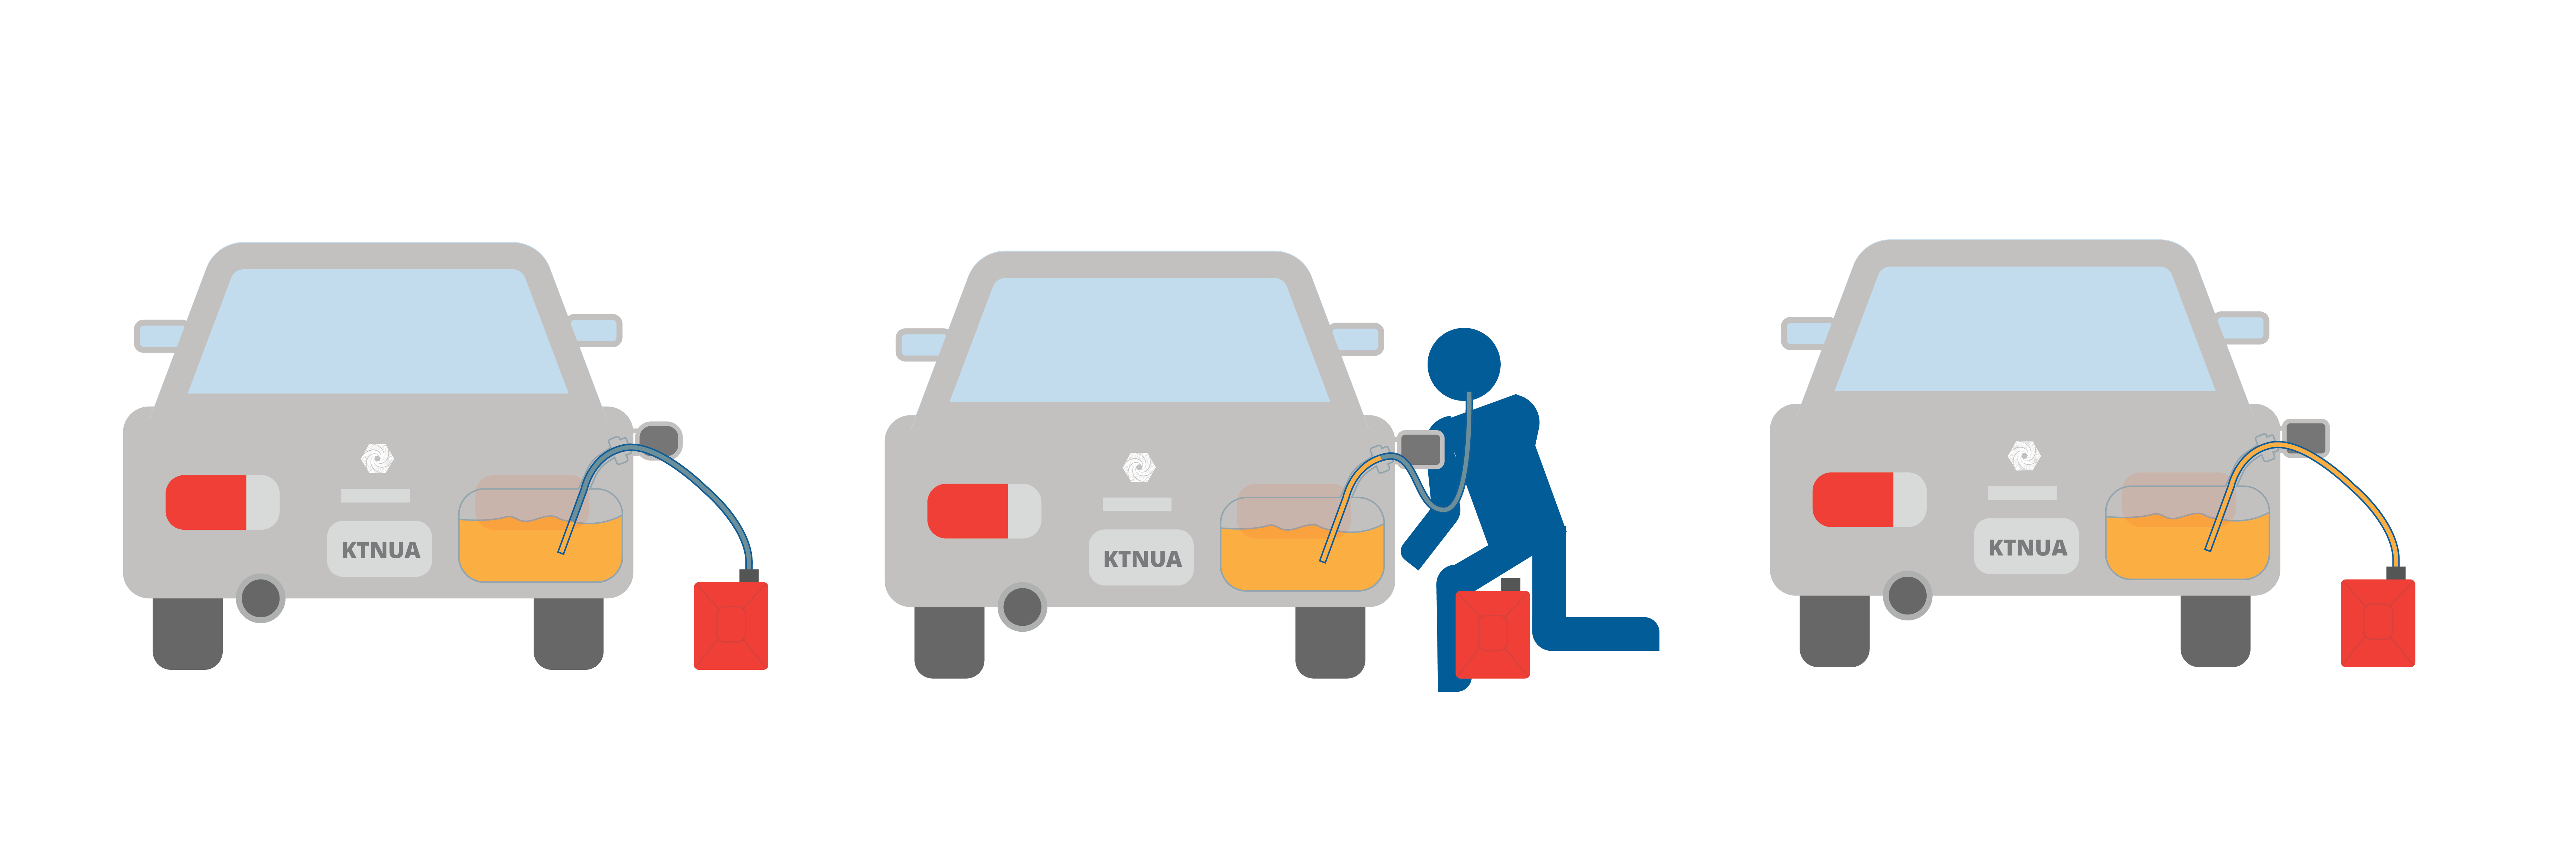
\includegraphics[width=\textwidth]{siphon.png}


\section{How a Toilet Works}

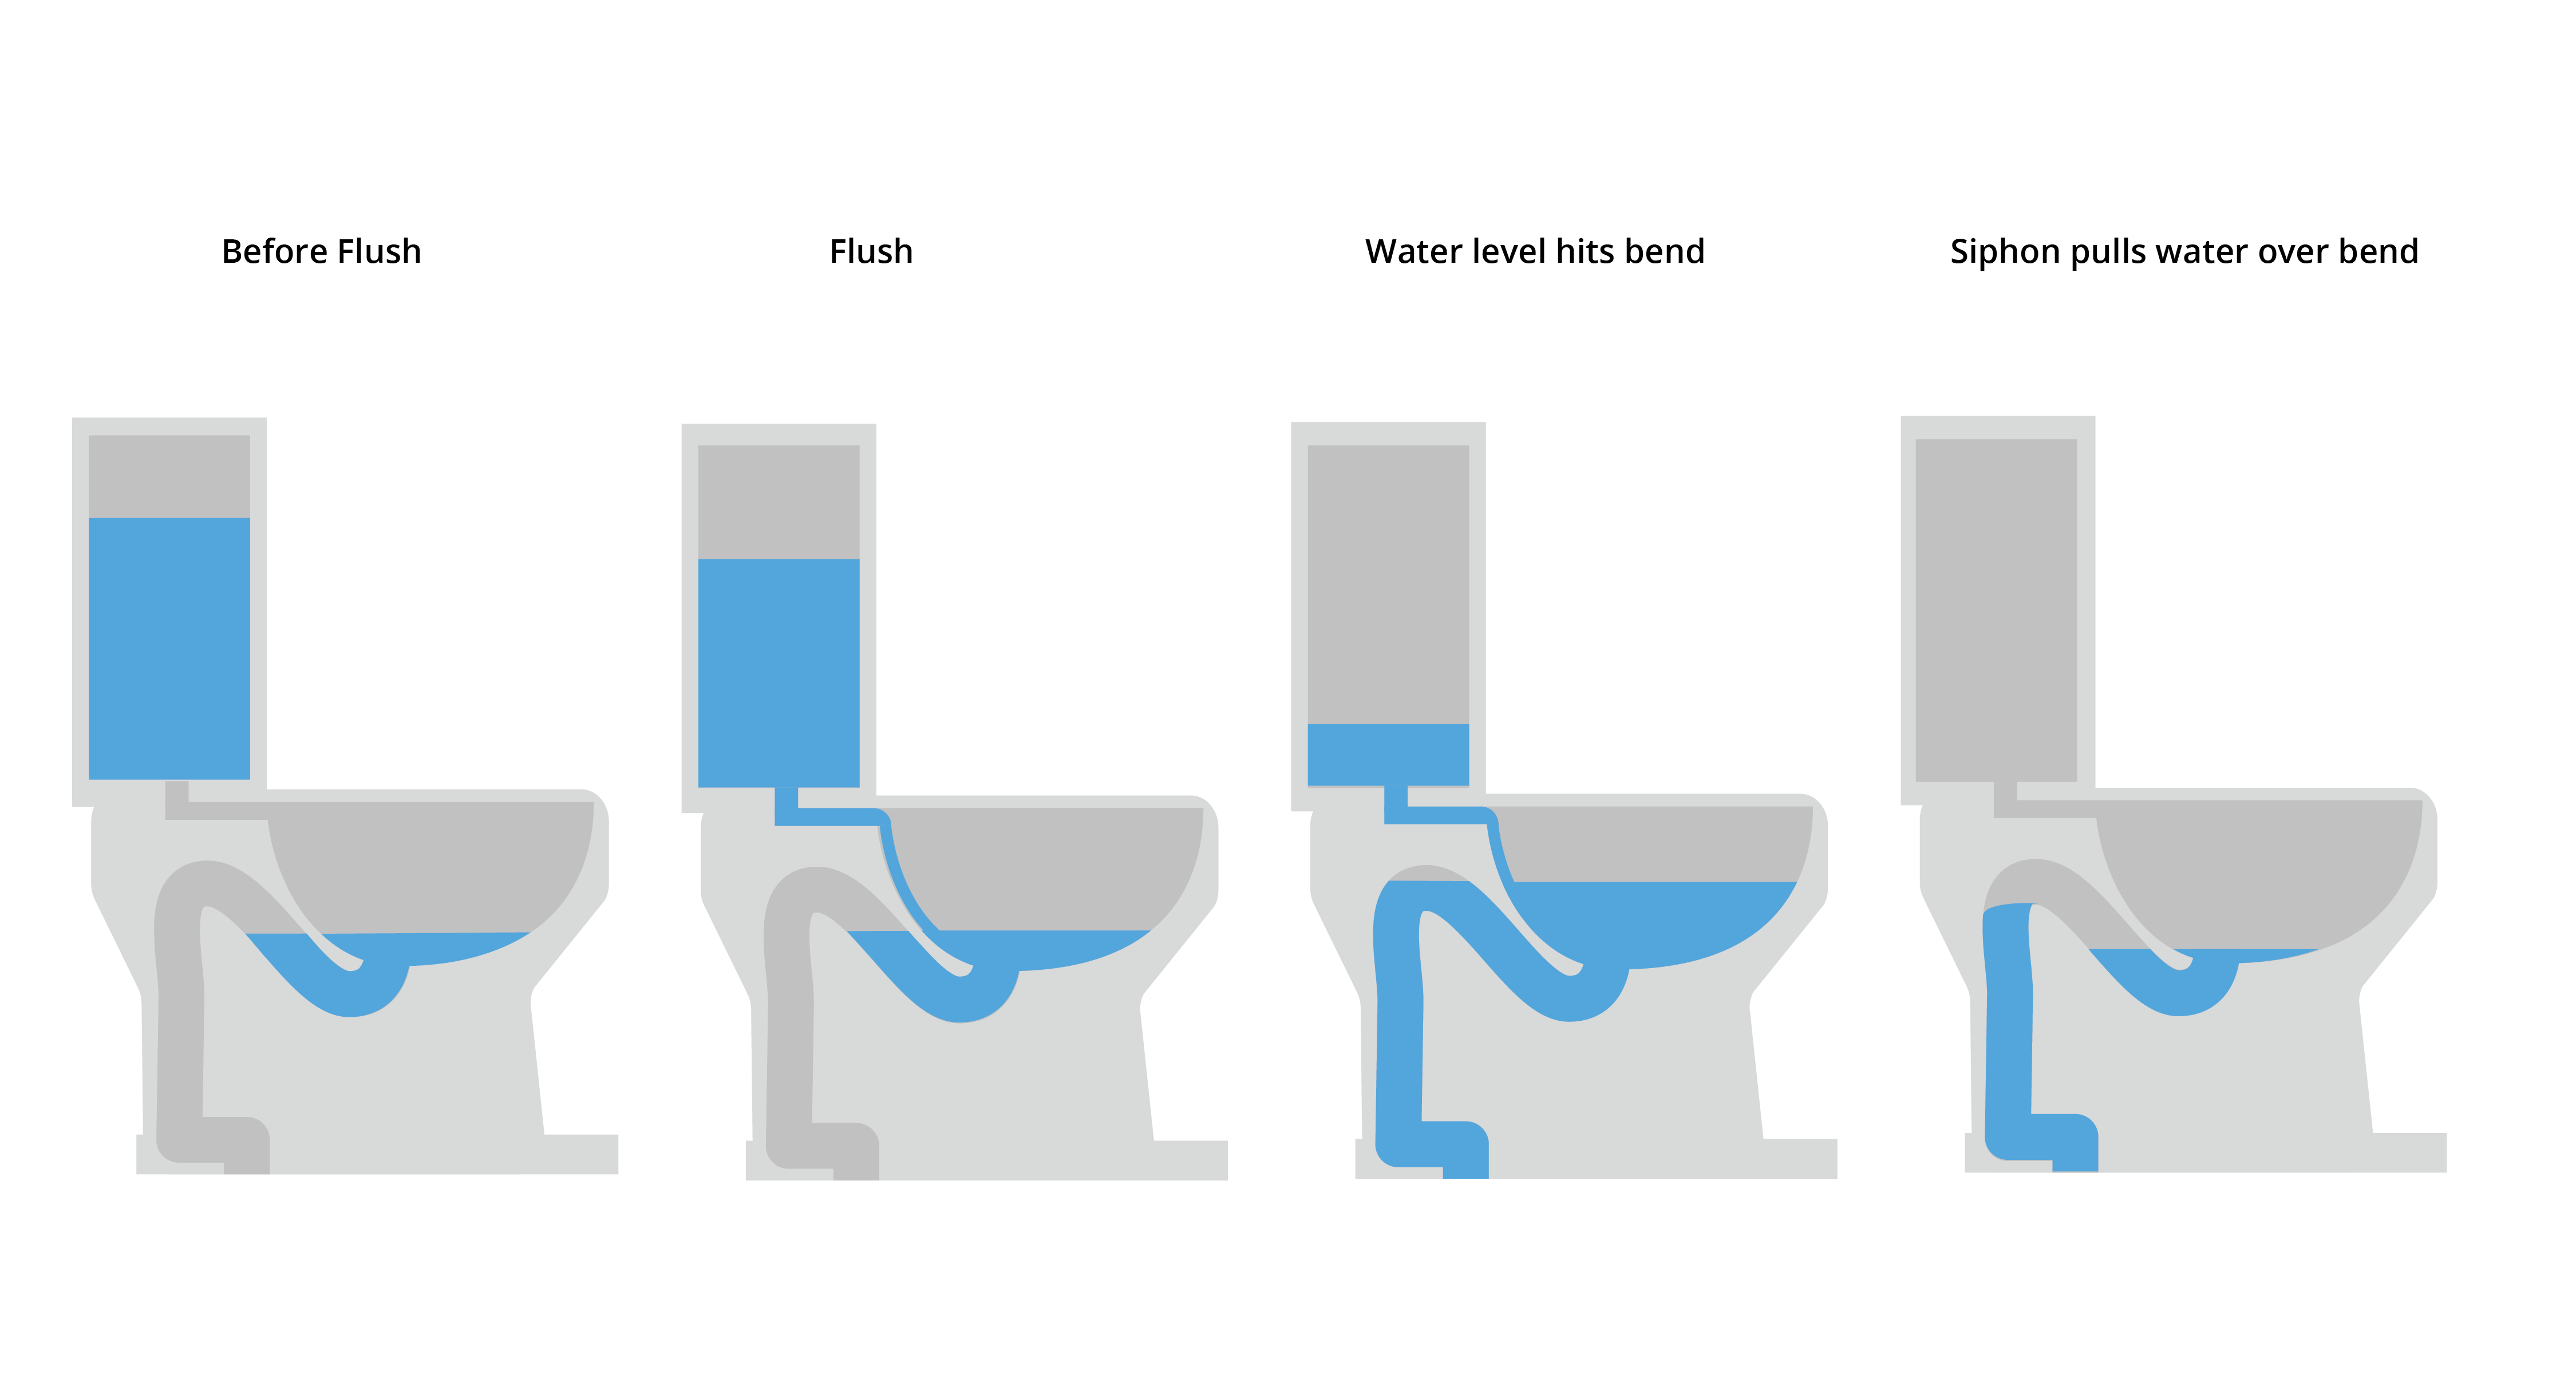
\includegraphics[width=\textwidth]{toilet.png}

